\documentclass[10pt]{article}
\usepackage{multicol}
\usepackage{authblk}
\usepackage{mathptmx}
\usepackage{graphicx}
\setlength{\columnsep}{5mm}
\usepackage{blindtext}
\usepackage{geometry}
\usepackage{url}
\usepackage{listings}
\usepackage{xcolor}
\usepackage{float}
\usepackage{longtable}
\usepackage{cite}


\definecolor{codegreen}{rgb}{0,0.6,0}
\definecolor{codegray}{rgb}{0.5,0.5,0.5}
\definecolor{codepurple}{rgb}{0.58,0,0.82}
\definecolor{backcolour}{rgb}{0.95,0.95,0.92}

\lstdefinestyle{mystyle}{
    backgroundcolor=\color{backcolour},   
    commentstyle=\color{codegreen},
    keywordstyle=\color{magenta},
    numberstyle=\tiny\color{codegray},
    stringstyle=\color{codepurple},
    basicstyle=\small,
    columns=flexible,
    breakatwhitespace=false,         
    breaklines=true,                 
    captionpos=b,                    
    keepspaces=true,                 
    numbers=left,                    
    numbersep=2pt,                  
    showspaces=false,                
    showstringspaces=false,
    showtabs=false,                  
    tabsize=2
}

\lstset{style=mystyle}

\geometry{
  a4paper,
  left = 20mm,
  top = 2mm,
  right = 20mm
}

\title{\textbf{Parallel dragonfly algorithm} %
  \\[2ex] \large High Performance Computing for Data Science course 2024/2025}

\author[1]{Mattia Santaniello}
\author[2]{Alessio Zeni}
\affil{University of Trento}

\begin{document}

\maketitle

\begin{multicols}{2}[
  \fontsize{9}{9}
  \section*{Abstract}
  \textbf{
    Dragonfly algorithm is an approach used to solve optimization problems through the emulation of dragonflies movements, but it lacks scalability.
  In this paper the authors propose an approach based on parallelization using dedicated libraries for high performance multiprocess applications like MPI, and OpenMP API for multithread parallelization.
  A comparison of execution times is then conducted between presented implementation and the classic approach based on serial programming,
  to determine whether parallelization leads to performance improvements and enables possible future extensions.
  }\newline]

\section{Introduction}
Swarm intelligence algorithms are inspired by the collective behavior of biological systems, where simple rules followed by individuals lead to the emergence of complex and adaptive group behavior. The concept was first introduced in Reynolds' Boids model (1987) \cite{TODO}, which simulated flocking behavior, and gained significant traction in Computer Science with the Ant Colony Optimization algorithm (1995) \cite{TODO}.
These algorithms are meta-heuristic in nature, leveraging decentralized and parallel exploration-exploitation strategies to solve optimization problems.

The dragonfly algorithm, first proposed in 2014 and published in 2015 \cite{DAReview}, is a bio-inspired optimization algorithm that simulates the behavior of dragonfly swarms.
By mimicking natural behaviors such as alignment, separation, cohesion, attraction to food sources, and distraction from enemies, the algorithm achieves a balance between exploration and exploitation.
This makes it particularly effective at navigating complex search spaces while reducing the likelihood of being trapped in local optima.
As of 2019, the algorithm has been cited in over 300 scientific papers, highlighting its impact and popularity in the field.

This paper focuses on parallelizing the dragonfly algorithm to improve its scalability and performance. Using popular parallel APIs such as OpenMP for multithreading and MPI for distributed memory systems, we aim to demonstrate how parallelization can significantly reduce execution time while maintaining the algorithm's effectiveness. The results of this study could pave the way for future research and applications of the dragonfly algorithm in high-performance computing environments.

\subsection*{How the algorithm works}
The execution of the dragonfly algorithm begins with the initialization of several arrays: the position vector $P$ representing the positions of all dragonflies, the step vector $\Delta P$ representing their velocities, the position of food sources $F$, and the position of enemies $E$. The algorithm then enters an iterative loop where, for each dragonfly, coefficients are calculated to update its internal state. These coefficients are derived from the observed behaviors of dragonflies in nature, which include:

\begin{itemize}
  \item \textbf{Alignment}: The tendency to match the velocity of neighboring dragonflies, calculated as:
  $$A_i = \frac{\sum_{j=1}^M V_j}{M},$$
  where $V_j$ is the velocity of the $j$-th neighbor and $M$ is the number of neighbors.

  \item \textbf{Separation}: The tendency to avoid collisions with other dragonflies, given by:
  $$S_i = -\sum_{j=1}^M (P - P_j),$$
  where $P_j$ is the position of the $j$-th neighbor and $P$ is the current dragonfly's position.

  \item \textbf{Cohesion}: The tendency to move toward the center of the group, expressed as:
  $$C_i = \frac{\sum_{j=1}^M P_j}{M} - P.$$

  \item \textbf{Attraction to food}: The tendency to move toward a food source, represented by:
  $$F_i = F^+ - P,$$
  where $F^+$ is the position of the food source.

  \item \textbf{Distraction from enemies}: The tendency to move away from enemies, modeled as:
  $$E_i = E^- + P,$$
  where $E^-$ is the position of the enemy.
\end{itemize}

\noindent Once these coefficients are calculated, the step vector $\Delta P$ for each dragonfly is updated using the formula:
$$\Delta P_i^{t+1} = sS_i + aA_i + fF_i + cC_i + \omega \Delta P_i^t,$$
where $s$, $a$, $f$, $c$, and $\omega$ are weights for separation, alignment, attraction, cohesion, and inertia, respectively. These weights are randomly chosen within the interval $[0,1]$. The new position of each dragonfly is then computed as:
$$P_i^{t+1} = P_i^t + \Delta P_i^{t+1}.$$

If a dragonfly has no neighbors, it is assumed to move randomly. This is modeled using a random walk function, often implemented as a Lévy flight:
$$P_i^{t+1} = P_i^t + \mathrm{Levy}(d),$$
where $d$ is the dimension of the position vector. The Lévy flight function is defined as:
$$\mathrm{Levy}(d) = 0.01 \times \frac{r_1 \times \sigma}{|r_2|^{1/\beta}},$$
where $r_1$ and $r_2$ are random numbers uniformly distributed in $[0,1]$, and $\sigma$ is calculated as:
$$\sigma = \frac{\sin\left(\frac{\beta \pi}{2}\right) \Gamma(1+\beta)}{\Gamma\left(\frac{\beta+1}{2}\right) \beta 2^{(\beta-1)/2}},$$
with $\Gamma(x)$ being the gamma function and $\beta$ a constant. Alternatively, Brownian motion can be used instead of Lévy flight, which has shown better performance in some cases \cite{BDragonfly}.



\section{General approach}
With the overall procedure outlined, we can now present a naive implementation of the dragonfly algorithm. This initial implementation serves as a foundational baseline for further optimization and parallelization. The following code snippet illustrates the core structure of the algorithm:

\begin{lstlisting}[language=C,caption={first implementation of the dragonfly algorithm}]
void dragonfly_algorithm(Dragonfly *d, 
                        float *average_speed,
                        float *cumulated_pos, 
                        float *food, 
                        float *enemy,
                        unsigned int N, 
                        unsigned int random_seed) {

  unsigned int dimensions = d->dim;
  float S;
  float A;
  float C;
  float F;
  float E;
  float levy;

  float *cur_pos;
  float *cur_speed;

  for (unsigned int j = 0; j < d->N; j++) {
    unsigned random = random_seed + j;
    cur_pos = d->positions + j * dimensions;
    cur_speed = d->speeds + j * dimensions;

    // compute speed = sSi + aAi + cCi + fFi + eEi + w

   for (unsigned int i = 0; i < dimensions; i++) {
      S = ((cumulated_pos[i] - cur_pos[i]) / (float)N);
      A = average_speed[i];
      C = (cumulated_pos[i] / (float)N) - cur_pos[i];
      F = food[i] - cur_pos[i];
      E = enemy[i] + cur_pos[i];
      levy = RAND_FLOAT(1.0, &random);

      cur_speed[i] *= d->w.w;
      cur_speed[i] += d->w.s * S;
      cur_speed[i] += d->w.a * A;
      cur_speed[i] += d->w.c * C;
      cur_speed[i] += d->w.f * F;
      cur_speed[i] += d->w.e * E;
      cur_speed[i] += levy;

      cur_pos[i] += cur_speed[i];
    }
  }
}
\end{lstlisting}

\noindent After initializing the velocities and positions of agents,
represented by two separate matrices with dimensions equal to the number of agents in the population times the problem's dimensionality, the algorithm begins its main execution loop.
This loop runs for a fixed number of iterations, stored in the variable $d\rightarrow N$.
During each iteration, the algorithm retrieves the position and velocity of the current dragonfly, represented by the pointers \textit{cur\_pos} and \textit{cur\_speed}, along with the cumulated coordinates of its neighbors.
The execution proceeds with the following steps:

\begin{itemize}
  \item Retrieve the current speed and position of the $j$-th dragonfly.
  \item Compute the separation, alignment, cohesion, food attraction, and enemy distraction vectors, storing them in local variables with their respective abbreviations.
  \item Calculate the product of the weights and the individual coordinates of the velocity array.
  \item Update the speed and position of the dragonfly, incorporating Brownian motion.
\end{itemize}

\noindent Notice that the computation of velocities and position updates is compacted into the same \textbf{for} loop.
This optimization reduces execution time by performing all calculations locally within the loop, eliminating the need for auxiliary arrays to store intermediate coefficients.
The rationale for dividing the separation coefficient by the number of neighbors will be explained later in this paper (TODO reference).

\section{Critical analysis of the coefficients}
During our implementation we discovered some ambiguities in the original paper:
\begin{itemize}
  \item In the original paper \cite{Original}, the term "neighbors" is used frequently without providing a precise definition.
  While a general distance metric, such as Euclidean distance, could be assumed, the paper also claims that the algorithm runs in linear time with respect to the number of dragonflies and the iteration count.
  This claim would not hold if Euclidean distance were used, as calculating the distance between each pair of dragonflies would result in a time complexity of $O(N^2)$. 

  A possible solution to achieve linear time complexity might involve using advanced geospatial algorithms, but we doubt this was the original intention of the authors.
  To address this ambiguity, we decided to divide the population into chunks and progressively merge these chunks until only one remains (as detailed in Section \ref{chunks}).
  This approach not only resolves the issue of defining neighbors but also mitigates the problem of premature convergence, which is common in swarm optimization algorithms.

  \item For the algorithm to be robust, it must ensure that no parameter values lead to divergence.
  As an initial solution, we introduced a \texttt{max\_speed} parameter that changes over time to ensure stability.
  However, since this parameter was not described in the original paper, we omitted it in later implementations. 

  This omission led to instabilities, particularly with the enemy coefficient (if it exceeded 0.5) and the separation coefficient.
  For example, the separation coefficient could cause exponential growth: if the distance between a dragonfly and the average position of the population is very small (e.g., 0.001) but there are many dragonflies in the neighborhood (e.g., 1000), the coefficient would become large (e.g., 1).
  In the next iteration, the dragonflies would move far from the center, causing the distance to grow exponentially.

  To address this, we modified the separation formula as follows:
  $$S_i = - \frac{\sum_{j=1}^M (P - P_j)}{M},$$
  where $M$ is the number of neighbors.
  This normalization ensures that the separation coefficient remains stable regardless of the number of neighbors.

  \item The enemy coefficient, as described in the original paper, does not behave as intended.
  Specifically, the sum of vectors does not necessarily point outward from the enemy (e.g., when position vectors are aligned).
  We assumed this was a typo, but even using the difference of vectors would not suffice.
  If the enemy is too close to the dragonfly, the difference vector would become smaller instead of larger, leading to incorrect behavior.

  A potential solution would be to normalize the difference vector by its length (i.e., use the inverse of the vector length).
  However, this formulation would deviate significantly from the original paper.
  As a result, we decided to retain the original formulation and evaluate its behavior empirically.

\end{itemize}


\subsection*{Chunk-based Optimization}
\label{chunks}
As mentioned earlier, the dragonfly algorithm, like many other swarm optimization solutions, has a high chance of getting stuck in local minima, limiting its ability to find better candidates.
One common approach to mitigate this issue in swarm algorithms is to avoid relying solely on Euclidean distance for neighborhood calculations.
Instead, the population can be divided into random groups, which are progressively merged over time until only one group remains.
This strategy allows for greater exploration in the early stages and focuses on exploitation as the algorithm converges.

In order to do that, and efficently, we divided the search space into chunks, with each thread processing an equal number of chunks.
Every $x$ iterations, these chunks are merged into larger logical chunks, each containing a power of 2 smaller chunks.
These logical chunks act as neighborhoods for the dragonflies. 

To share the contributions of each chunk, we used a modified butterfly algorithm where the contributions from all elements in a chunk is shared across all the relevant threads.
As an optimization, if a chunk is entirely contained within a single thread, the contributions are shared locally without inter-thread communication. 

Figure \ref{fig:chunks} illustrates the communication process.
The circles represent different chunks, and the colors represent logical chunks.
The blue arrows indicate communication within a process, while the red arrows represent communication across processes.

\begin{figure}[H]
  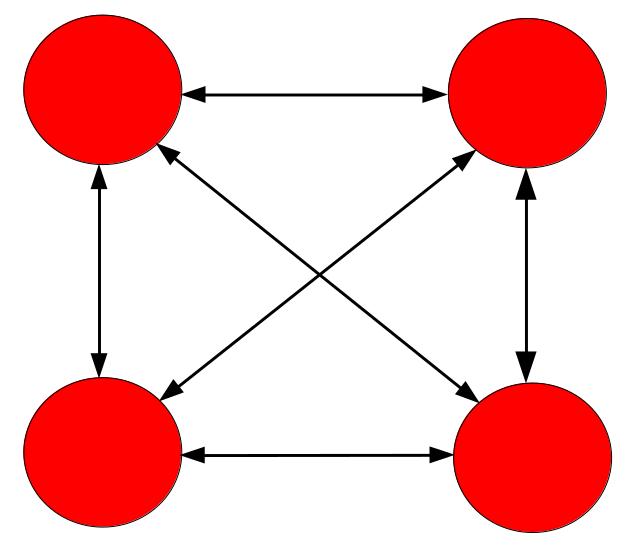
\includegraphics[scale=0.21]{img/chunks.png}
  \centering
  \caption{Illustration of communication between chunks.}
  \label{fig:chunks}
\end{figure}

\subsection*{Chunk-based Optimization Version 2}

To improve the previous algorithm, we simplified the chunk structure by removing the first chunk block abstraction.
This modification ensures that there is only one type of chunk, eliminating an unnecessary layer of abstraction, and decreasing the risk of off by one error.
In Figure~\ref{fig:chunks}, the circles now represent butterflies, and the colors correspond to logical chunks.

Additionally, we modified the communication algorithm to address a limitation of the butterfly algorithm, which requires the number of participating threads to be a power of two.
To overcome this constraint, we implemented a two-step approach: first, contributions are accumulated into a single element, and then the result is shared with all participating processes.
This approach ensures compatibility with any number of threads while maintaining efficient communication.





\section{Parallelization with MPI}

The Message Passing Interface (MPI) is a portable message-passing standard designed to function on parallel computing architectures.
For our implementation it is usefull because it let us to express multiprocess comunication across multiple machines.

\subsection*{MPI on chunks}
By far the biggest challenge in the parallelization with MPI was the comunication of the chunks partial computations (given that a chunk may or may not span multiple process).
Mpi has an atomic function called $sendrecv$, that permits to send a message from a thread while receving from (possibly) another thread.
This is super useful, but it could have caused deadlocks if every process has to comunicate with multiple chunks.
So in order to use that we needed to ensure that each process is responsible of the accumulation of one chunk.
We did this by ensuring that if a chunk starts in another process, and ends in this one, the process comunicate its contribute to the left process. Then the accumulation is performed and the result is shared back to the current block.

\begin{figure}[H]
  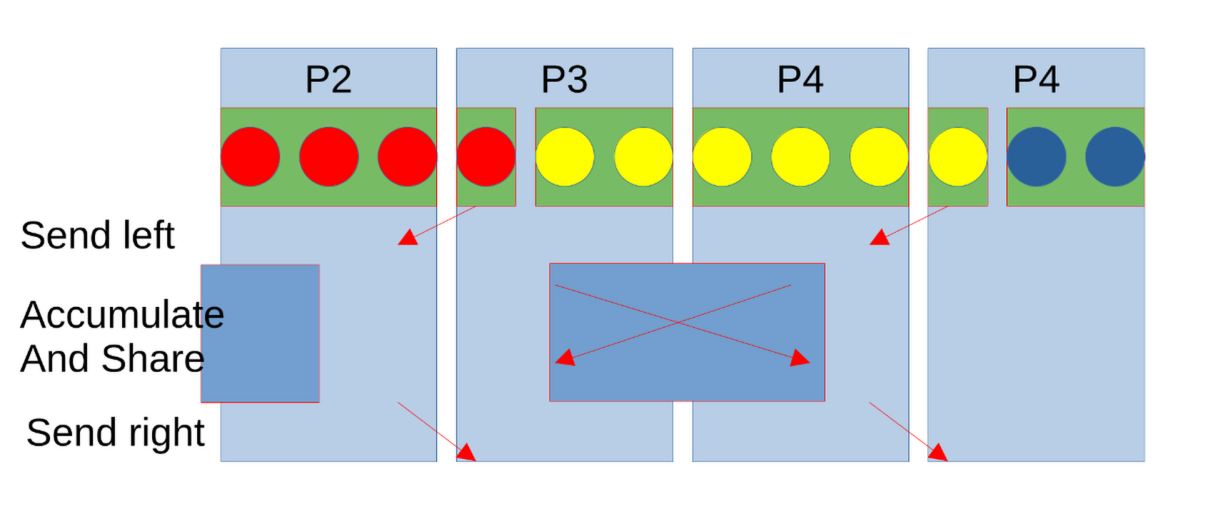
\includegraphics[scale=0.25]{img/MPI.png}
  \centering
  \caption{Illustration of communication between processes}
  \label{fig:MPI}
\end{figure}

The algorithm is divided in steps (isolated by an MPI barrier):
\begin{itemize}
  \item \textbf{Send left}: first, the process that have the end of a block, share theyr contribute to the left
  \item \textbf{Accumulate and share} Then it is accumulated in the first process and broadcasted back to all partecipating processes
  \item \textbf{Send right} Then the rightmost process in the block receives the accumulated value from the left.
\end{itemize}

In this way the comunication is efficient, and looking at the results it scales very wheel. More on that in section \ref{results}.


\subsection*{MPI and training}
Since the parallelization with MPI is highly efficient, it becomes feasible to refine the hyperparameters of small problem instances by scaling the computation across hundreds of cores.
In the results section, we demonstrate how the hyperparameters for smaller instances of the dragonfly algorithm were trained on a shifted and rotated Rastrigin function, which is commonly used as a benchmark for optimization algorithms.

The learned hyperparameters were then fed back into the algorithm to enhance its performance.
This iterative process was repeated twice, allowing the algorithm to progressively improve its ability to navigate complex search spaces.
By leveraging the scalability of MPI, we were able to significantly reduce the time required for hyperparameter tuning while maintaining the accuracy of the results.

\section{OpenMP implementation}

OpenMP is a low level API that allows us to execute a sequence of instructions on different threads belonging
to the same CPU core, improving in this way the performances of our implementation. This feature can be used to 
speed up the execution of some slow functions, in our case these will be dragonfly-compute-step and message-accumulate

\subsection*{General use}

First of all it is necessary to understand how OpenMP should be inserted in the code: first of all we have to use 
a compiler that supports this technology, in our case we have gcc, which allows OpenMP execution thanks to the flag -fopenmp.
Second we need to include a pragma directive in our code, which will wrap the set of instructions that we are interested to execute
in parallel. Since the implemented results will perform loops mainly then it is fundamental to calculate the work balance between the number of iterations, if the main
body is a loop,
and the number of threads available. Each thread has to define the starting and the end point of the loop that has to execute,
calculating the starting index as $rank*ratio$ and the end one as $ratio*(rank+1)$, where $rank$ is the ID of the thread

\subsection*{dragonfly-compute-step}

One of the two functions that we are interested to execute using OpenMP is \textit{dragonfly-compute-step}:
if we take a look on the serial version we notice that each computation step is independent
from other iterations. This means that the execution flow can be split in many subtasks assigned
to threads. The following code snippet illustrate how all the procedure has been implemented

\begin{lstlisting}[language=C,caption={parallelized dragonfly-compute-step}]
void dragonfly_compute_step(Dragonfly *d, 
                            float *average_speed,
                            float *cumulated_pos, 
                            float *food, 
                            float *enemy, 
                            unsigned int N, 
                            unsigned int NR_THREADS) {

  unsigned int base_random = rand_r(&d->seed);
  unsigned int rest = d->N % NR_THREADS;
  unsigned int ratio = d->N / NR_THREADS;

  ...

  #pragma omp parallel num_threads(NR_THREADS)
    {
      
      unsigned int rank = omp_get_thread_num();
      //printf("rank=%d\n", rank);
      unsigned int base = ratio * rank;
      unsigned int limit = ratio * (rank + 1);
      inner_dragonfly_step(d, average_speed, 
                          cumulated_pos, food, 
                          enemy, N,
                          base, limit, base_random);
    }
  
  ...

  if (rest != 0) {
      unsigned int r_base = ratio * NR_THREADS;
      unsigned int r_end = d->N;

      inner_dragonfly_step(d, average_speed, 
                           cumulated_pos, 
                           food, enemy, N,
                           r_base, r_end, base_random);
    }
  }

  weights_step(&d->w);
  
  }

\end{lstlisting}


\noindent After we got all basic informations the \textit{inner\_dragonfly\_step}
function can be executed, wrapping it into the \textbf{pragma} directive that we have seen earlier: in this way each thread will 
perform the necessary operations only on a specific portion of the overall positions and speeds arrays.
If the number of threads does not divide perfectly the size of the arrays then we compute the rest
returned from the ratio calculation and the remaining cells will be processed using the serial approach.

\subsection*{computation\_accumulate}

The \textit{computation\_accumulate}  must compute
the cumulated positions and speeds of the chunk and find the best food and enemy positions.
The implementation of a parallelized approach in this case  is more complicated to achieve, 
because threads should read and write on the same memeory areas which could be 
difficult to execute independently from each other. This time it is necessary to define
local buffers for each thread, so they can store temporary results without the risk of using
overlapping memeory locations. 
\begin{figure}[H]
  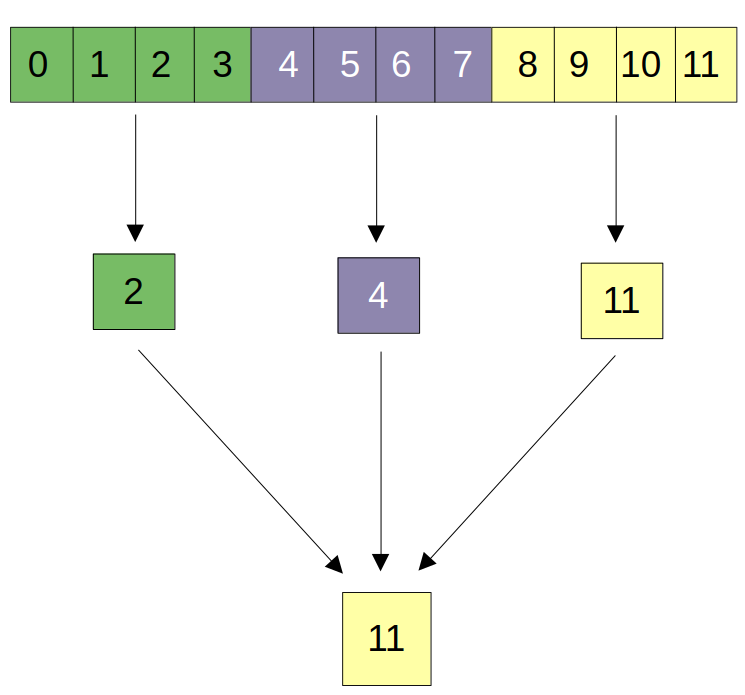
\includegraphics[scale=0.2]{img/reduce-example.png}
  \centering
  \caption{Illustration of the reduce process performed by the computation\_accumulate function}
\end{figure}
\noindent The parallel section provides that each thread must compute the local
cumulated sums of velocities and positions, then they must select the position with the best fitness value
in order to find the best local position of food and enemies. Once the local execution is completed
it will update the global status of the chunk using a critical section, with one thread that can execute that
specific portion of the program

\section{Final execution and results}
Now that we have described all the procedure it is time to illustrate how 
the algorithm has been executed. This job has been performed by the
High Performance Computing cluster at University of Trento, which 
use a particular technology called PBS to handle multiple tasks at the same
time: this feature comes useful in our case since, as we will see later, we 
execute multiple istances of the same problem
\subsection*{structure of the execution}

As anticipated we will execute the same problem using multiple instances with different amount of
resources in order to get a complete evaluation of performance. The overall execution use from 1 to 8
threads, and 4 to 1024 cores

\subsection*{performace theory}

After the end of all tasks it is possible to check how much gain in performance we have obtained.
To do this it is necessary to introduce some theoretical concepts that will give us the tools that
will give us a good metric system to evaluate our results.Speedup is defined as the ratio between the the execution times of the serial and parallel
implementations, so the formula will be equal to: $$Speedup = \frac{T_{serial}}{T_{parallel}}$$ 
from this definition it is obvious that the more the speedup is the more the parallel implementation
performs better. There is a particular case where the time execution of the denominator can be defined
as $T_{parallel}=T_{serial}/p$, where \textit{p} is the number of cores: this is called \textit{linear speedup},
and in this situation it perfectly match with the classic speedup coefficient
Efficiency is another important parameter, and it is defined by the ratio of the speedup and the 
number of cores, giving the following formula: $$E = \frac{Speedup}{p}$$
also in this case the efficiency decrease due to the increase of the number of cores. In case
of linear speedup we get that the efficiency is equal to the inverse of $p$
\subsection*{results}
\label{results}
Now it is possible to show results obtained from the cluster,
using the configuration with 4 cores and 1 thread will be considered
equal as the serial time. The reason for this approach is that a single core computation would require 1024 times the workload of the 1024 process version, but we calibrated the 1024 core version to take 3 minutes.


\begin{tabular}{| c | c | c | c | c | c | c |}
  \hline
  T/p & 4	 & 8	& 16	& 32	& 64 & 128  \\
  \hline
  1 & 1	& 2,03 & 3,87 & 7,94 & 14,76 & 31,19  \\
  2 & 1,04 & 2,05 & 3,97 & 8,50 & 16,43 & 27,90 \\	
  4 & 1,01 &2,03	& 4,21 &	8,04 &	16,37 &	35,26	\\	
  8 & 1,02  &2,02 &	4,02 &	8,62 &	18,32 &	32,26 \\
  \hline
\end{tabular}
\newline\newline As we can see the speedup tends to 
increase when the number of cores increase, however when
we use more threads it happens that the
speedup start to decrease at a certain point for some
core configuration. As we can see from the plots it 
seems there are threshold at some specific points, depending
on the number of threads used; notice how the inclinations
of the lines in the plot tends to be less and less evident.

\begin{figure}[H]
  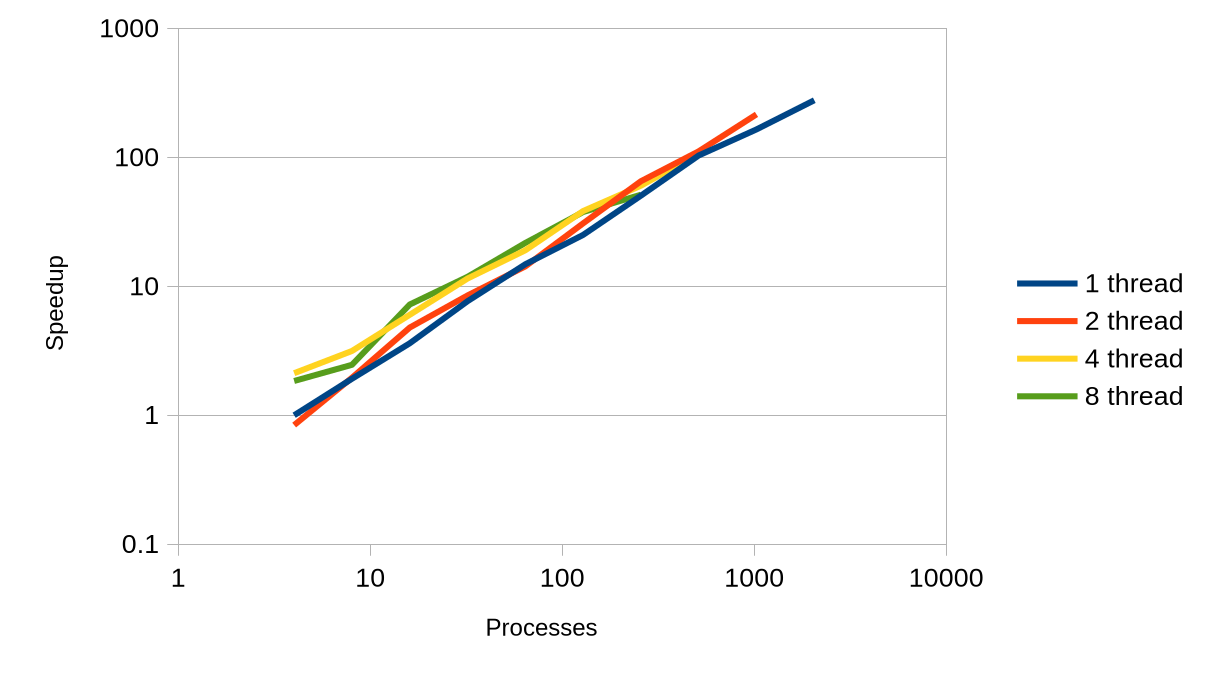
\includegraphics[scale=0.3]{img/speedup.jpg}
  \centering
  \caption{speedup graphic}
\end{figure}

\noindent 
Efficiency tends to present an unpredictable behaviour,
in fact the coefficients grows for some particular setups,
for others instead numbers decrease. If we take a look on
the plot below it shows that there is a high variance in the
datas, with the lines that tends to be more stretched when the
number of threads gets higher
\newline
\newline
\begin{tabular}{| c | c | c | c | c | c | c |}
  \hline
  T/p & 4	 & 8	& 16	& 32	& 64 & 128  \\
  \hline
  1 & 1	& 1,02 & 0,97 & 0,99 & 0,92 & 0,97  \\
  2 & 1,04 & 1,03 & 0,99 & 1,06 & 1,03 & 0,87 \\	
  4 & 1,01	&1,01&	1,05&	1&	1,02&	1,1	\\	
  8 &1,02&	1,01&	1,01&	1,08&	1,15&	1,01 \\
  \hline
\end{tabular}

\begin{figure}[H]
  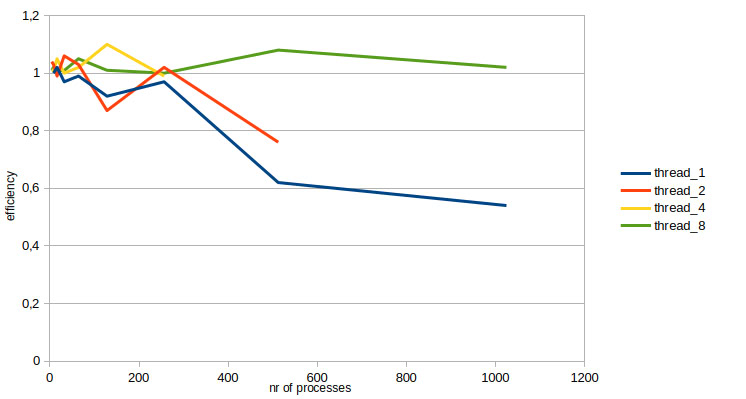
\includegraphics[scale=0.3]{img/efficiency.jpg}
  \centering
  \caption{efficiency graphic}
\end{figure}

\end{multicols}

\bibliographystyle{unsrt}
\bibliography{references}


\end{document}
